\documentclass[aspectratio=169]{beamer}
\usepackage[utf8]{inputenc}
\usepackage[T1]{fontenc}

\usetheme{focus}
\definecolor{main}{RGB}{11, 93, 25}

\usecolortheme[RGB={11,93,20}]{structure}
\usepackage[spanish]{babel}

\usepackage{colortbl}
\usepackage{color}
\usepackage{pifont}
\usepackage{ulem}



\usepackage{colortbl}
\usepackage{color}
\usepackage{pifont}
%\usepackage[normalem]{ulem}
\usepackage{listings}

\parskip=12pt

\lstset{basicstyle=\normalsize,
aboveskip=5pt,
basicstyle=\small\ttfamily,
belowskip=5pt
}

\author{Alberto Molina Coballes}
\title{Storage Area Network (SAN)}
\institute{IES Gonzalo Nazareno}
\titlegraphic{
\includegraphics[width=1.5cm]{cc_by_sa.png}}
\logo{
\includegraphics[width=.75cm]{logo_iesgn.png}}
\date{\today}

\definecolor{verde}{rgb}{0,0.73,0}

\begin{document}

\def\braces#1{[#1]}

\begin{frame}[t,plain]
\titlepage
\end{frame}

\begin{frame}
  \frametitle{Redes de almacenamiento}
  \begin{itemize}
  \item Red dedicada de almacenamiento que proporciona dispositivos de
    bloques a los servidores
  \item Los elementos típicos de una SAN son:
    \begin{itemize}
    \item Red dedicada alta velocidad (cobre o fibra óptica)
    \item Equipos o servidores que proporcionan el almacenamiento
    \item Servidores que utilizan los dispositivos de bloques
    \end{itemize}
    \item Los protocolos más utilizados son
      \href{https://en.wikipedia.org/wiki/ISCSI}{iSCSI} y
      \href{https://en.wikipedia.org/wiki/Fibre\_Channel\_Protocol}{Fibre
        Channel Protocol (FCP)}
  \end{itemize}
\end{frame}

\begin{frame}
  \frametitle{Elementos de Fibre Channel}
  \begin{columns}
    \column{0.5\textwidth}
    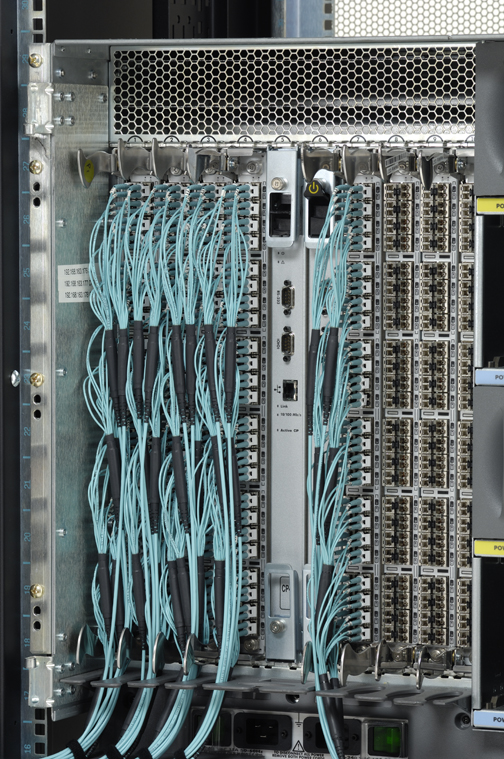
\includegraphics[width=.6\textwidth]{img/Fibre_Channel_Director.jpg}
    \column{0.5\textwidth}
    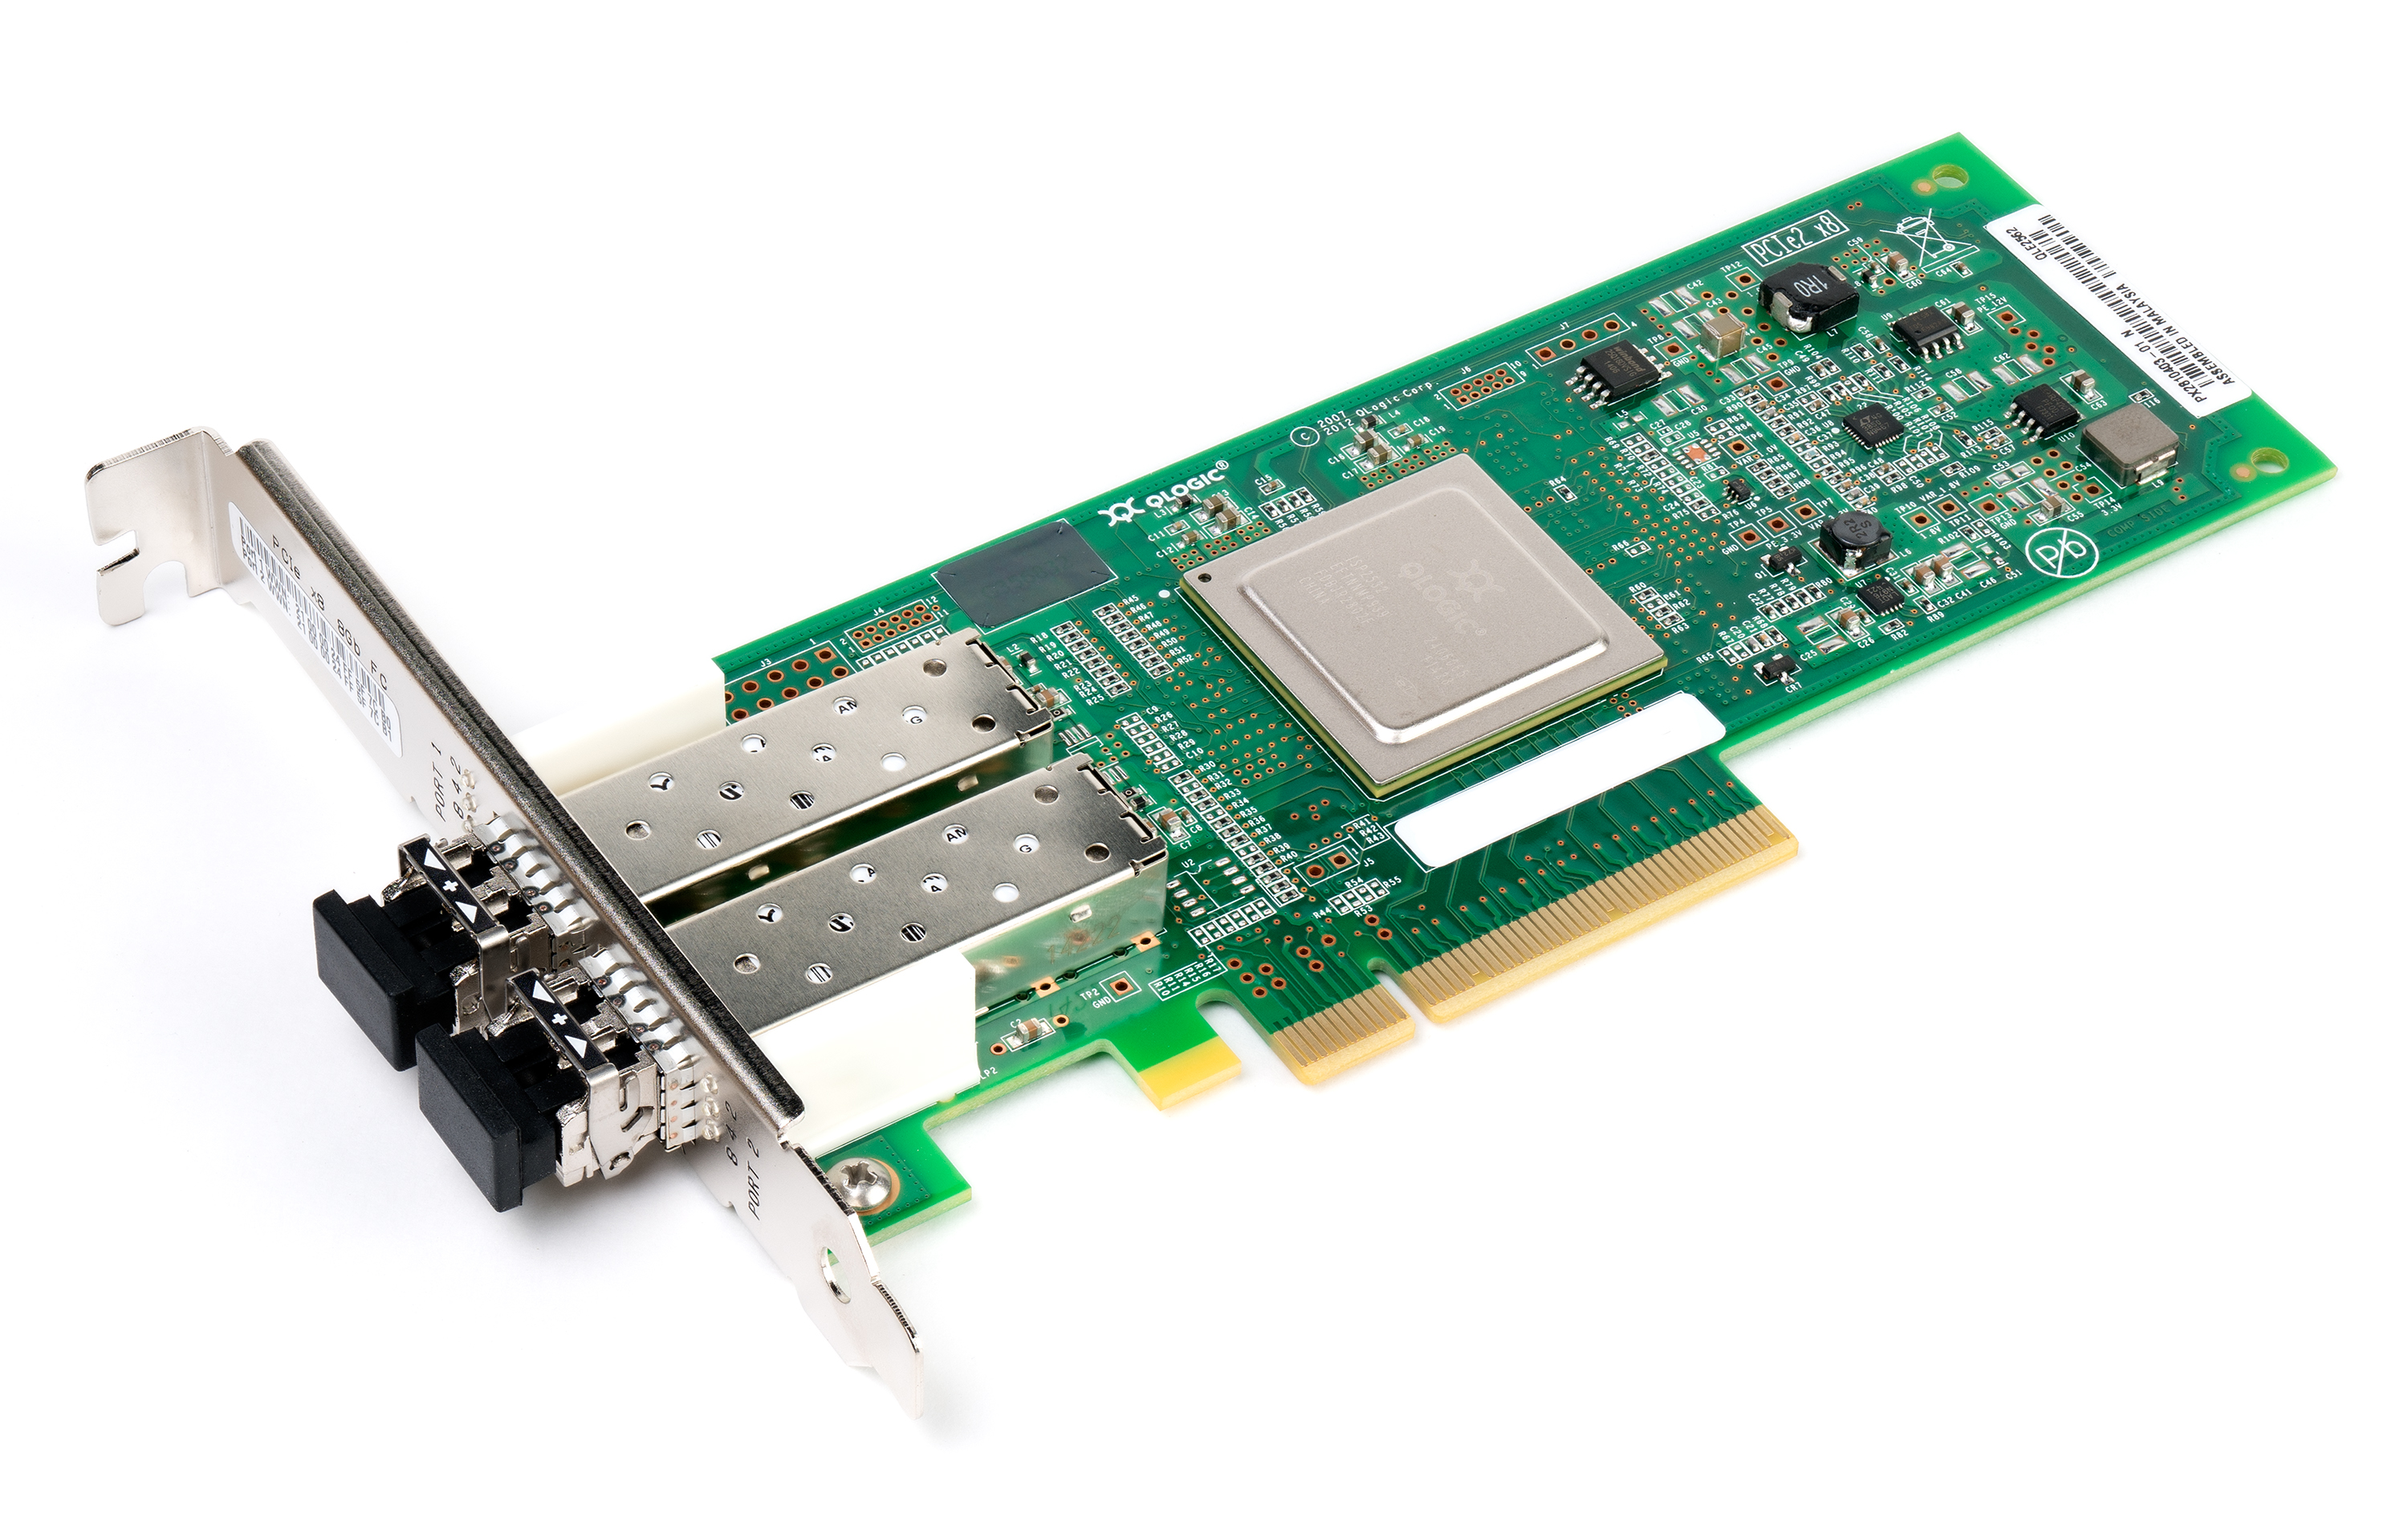
\includegraphics[width=\textwidth]{img/QLogic_QLE2562_8Gb_FC_HBA.jpg}
  \end{columns}
  Fuente: \href{https://en.wikipedia.org/wiki/Fibre\_Channel}{Wikipedia: Fibre Channel}
\end{frame}

\begin{frame}
  \frametitle{Esquema de SAN}
  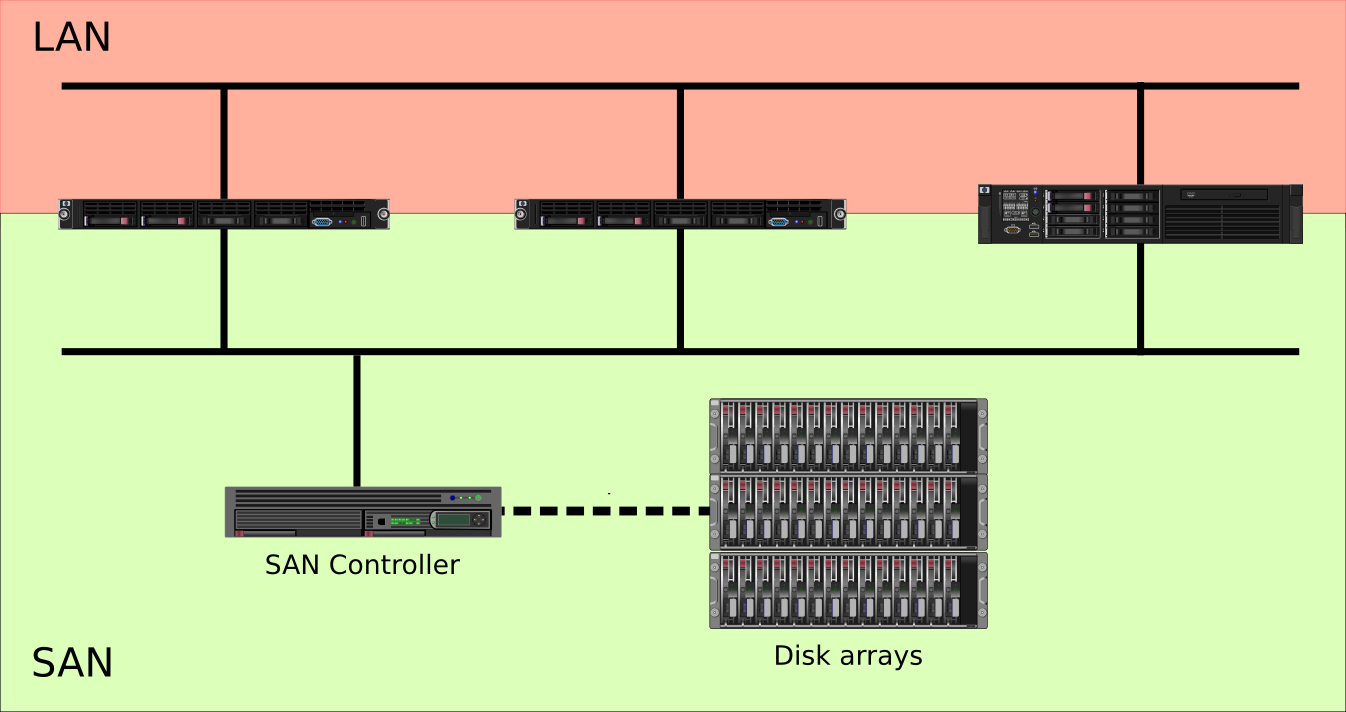
\includegraphics[width=\textwidth]{img/san.png}
\end{frame}
\end{document}
